\chapter{Convolutional layer}

\subsection*{Structure}

\begin{itemize}
\item Accepts a volume of size $W_1 \times H_1\times D_1$
\item Requires four hyperparameters:
\begin{itemize}
    \item Number of filters $K$
    \item their spatial extent $F$
    \item the stride $S$
    \item the amount of zero padding $P$
\end{itemize}
\item Produces a volume of size  $W_2 \times H_2 \times D_2$  where:
\begin{itemize}
    \item $W_2 = \frac{W_1-F+2P}{S+1}$
    \item $H_2 = \frac{H_1-F+2P}{S+1}$
    \item $D_2 = K$
\end{itemize}
\item With parameter sharing, it introduces $FFD_1$ weights per filter, for a total of $FFD_1K$ weights and $K$ biases.
\item The filters depth is always equal to the input volume depth.
\item The output volume depth is equal to the number of filters
\item In the output volume, the d-th depth slice (of size $W_2 \times H_2$ is the result of performing a valid convolution of the d-th filter over the input volume with a stride of $S$, and then offset by d-th bias.
\item Normally, in the same conv layer, all filters have the same dimensions so that special optimized routines can be invoked.
\end{itemize}

\subsection*{Explanation}
In a convolution layer we have filters. Each filter is a weight matrix which is convoluted over the input volume. Each time the filter is applied it outputs a single value. The result of convolving the filter over all the input volume is another volume called activation map. A filter's depth is always equal to the input volume depth. You can imagine a filter as a neuron.

\begin{figure}[h]
  \centering
  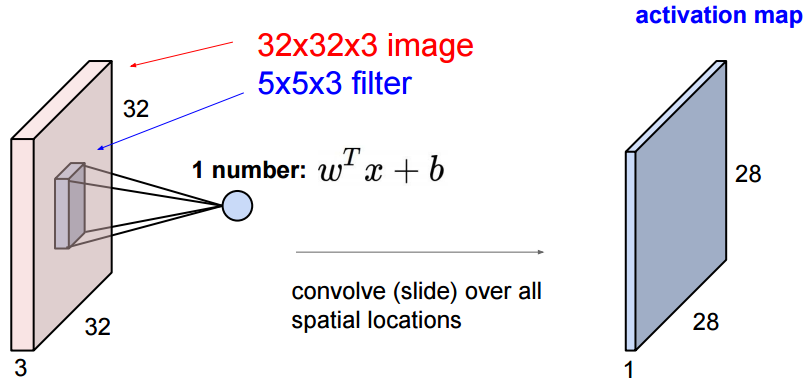
\includegraphics[width=0.4\textwidth]{Images/conv_layer/1.png}
  \caption{Convolution filter}
\end{figure}

Instead of having only one filter, we have a stack of filter which produce a stack of activation maps (one for each filter). In this example this conv layer has a stack of 6 filters ($5 \times 5 \times 3$). All positions in the same activation map share the same weights (filter)

\begin{figure}[h]
  \centering
  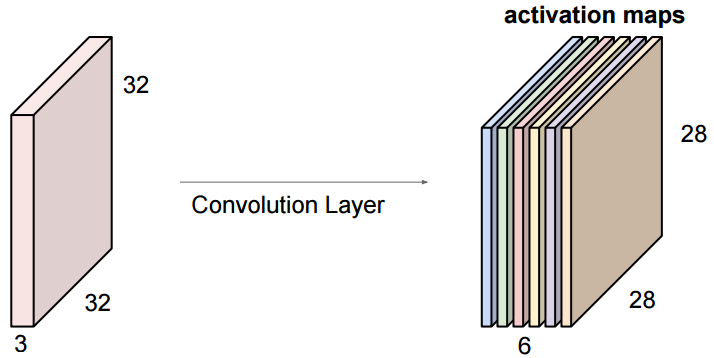
\includegraphics[width=0.4\textwidth]{Images/conv_layer/2.png}
  \caption{6 convolution filters output}
\end{figure}

\begin{figure}[h]
  \centering
  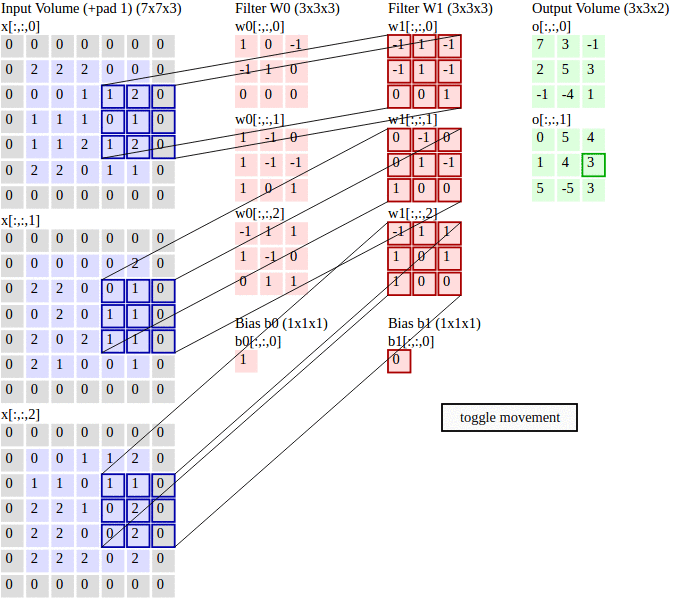
\includegraphics[width=0.5\textwidth]{Images/conv_layer/5.png}
  \caption{Example of a conv layer with 2 filters ($3 \times 3 \times 3$) over an input volume of ($7 \times 7 \times 3$) with 1 padding, which produces and output map of ($3 \times 3 \times 2$)}
\end{figure}

\begin{figure}[h]
  \centering
  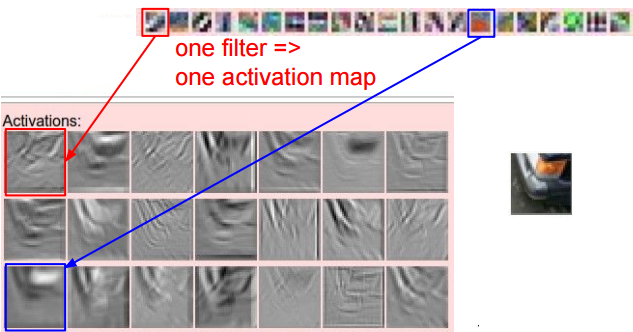
\includegraphics[width=0.4\textwidth]{Images/conv_layer/3.png}
  \caption{Example of the activation maps produced in a convolution layer. The small images on top are the stack of filters, the image on the right the input volume, and the grey-scale images the activation maps. White corresponds to high activations and black to low activations. Notice for example, that the filter marked in blue has an orange part, so when you slide this filter through the input image there are a lot of high activations in the area corresponding to the orange part of the input image. The output of this convolutional layer is going to be a stack of all these activation matrices.}
\end{figure}

\paragraph*{Padding} Add zeros around the input volume. The output volume decreases after each conv layer, so if we would not pad, the size of the activation maps will decrease very fast and after a few layers the volume would be $1 \times 1 \times ?$. This behavior is not desired because in deep learning we want to have a lot of layers. Why padding with zeros and not an extension of the image for example? Because in this way the padded cells do not contribute to the filter.

\paragraph*{Choosing hyperparameters} Should be using small filters (e.g. $3 \times 3$ or at most $5 \times 5$), using a stride of $S=1$, and crucially, padding the input volume with zeros in such way that the conv layer does not alter the spatial dimensions of the input. A common setting of the hyperparameters are: $F=3,S=1,P=1$; $F=5,S=1,P=2$; $F=5,S=2,P=?$and $F=1,S=1,P=0$. $K$ is usually a power of two value (e.g. 32,64,128,512) because libraries normally have optimized routines. If you must use bigger filter sizes (such as $7 \times 7$ or so), it is only common to see this on the very first conv layer that is looking at the input image. For a general $F$, it can be seen that $P=(F-1)/2$ preserves the input size.

\paragraph*{Parameter sharing} In an activation map, all the positions (neurons) share the same weights (filter). It makes sense to share weights because for example if the filter is searching for edges, it makes sense that it search edges in all the image. Moreover, sharing weights spatially avoids over-fitting the filter. It also helps reducing the number of parameters.

\paragraph*{Backpropagation} The backward pass for a convolution operation (for both the data and the weights) is also a convolution (but with spatially-flipped filters). This is easy to derive in the 1-dimensional case with a toy example (not expanded on for now).

\paragraph*{$1 \times 1$ convolution} As an aside, several papers use $1 \times 1$ convolutions, as first investigated by Network in Network. Some people are at first confused to see $1 \times 1$ convolutions especially when they come from signal processing background. Normally signals are 2-dimensional so $1 \times 1$ convolutions do not make sense (it’s just pointwise scaling). However, in ConvNets this is not the case because one must remember that we operate over 3-dimensional volumes, and that the filters always extend through the full depth of the input volume. For example, if the input is [$32 \times 32 \times 3$] then doing $1 \times 1$ convolutions would effectively be doing 3-dimensional dot products (since the input depth is 3 channels).

\paragraph*{Dilated convolutions} A recent development (e.g. see paper by Fisher Yu and Vladlen Koltun) is to introduce one more hyperparameter to the CONV layer called the dilation. So far we’ve only dicussed CONV filters that are contiguous. However, it’s possible to have filters that have spaces between each cell, called dilation. As an example, in one dimension a filter w of size 3 would compute over input x the following: \texttt{w[0]*x[0] + w[1]*x[1] + w[2]*x[2]}. This is dilation of 0. For dilation 1 the filter would instead compute \texttt{w[0]*x[0] + w[1]*x[2] + w[2]*x[4]}; In other words there is a gap of 1 between the applications. This can be very useful in some settings to use in conjunction with 0-dilated filters because it allows you to merge spatial information across the inputs much more agressively with fewer layers. For example, if you stack two 3x3 CONV layers on top of each other than you can convince yourself that the neurons on the 2nd layer are a function of a $5 \times 5$ patch of the input (we would say that the effective receptive field of these neurons is $5 \times 5$). If we use dilated convolutions then this effective receptive field would grow much quicker.

\subsection*{The power of small filters}
\begin{figure}[h]
  \centering
  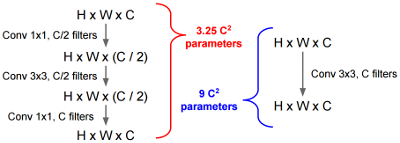
\includegraphics[width=0.5\textwidth]{Images/conv_layer/4.png}
  \caption{Network in network}
\end{figure}

3 Conv layers of $3 \times 3$ filters have the same receptive field as a 1 Conv layer of $7 \times 7$ filters. But lets compare both options:

Suppose input is $H \times W \times C$ and we use convolutions with $C$ filters to preserve depth (stride 1, padding to preserve $H$, $W$)

\begin{itemize}
\item three CONV with $3 \times 3$ filters
\begin{itemize}
\item Number of weights: $3 \times C \times (3 \times 3 \times C) = 27C^2$
\item Number of multiply-adds: $3 \times (H \times W \times C) \times (3 \times 3 \times C) = 27 HWC^2$
\end{itemize}
\item one CONV with $7 \times 7$ filters
\begin{itemize}
\item Number of weights: $C \times (7 \times 7 \times C) = 49C^2$
\item Number of multiply-adds: $(H x\times W \times C) \times (7 \times 7 \times C) = 49HWC2$
\end{itemize}
\end{itemize}


So 3 Conv layers of $3 \times 3$ filters have the same receptive field of a larger Conv layer of $7 \times 7$ filters but have a lower computation and memory complexity. Moreover, if we have ReLU layers after each Conv layer the 3 Conv layer option is more nonlinear (good).

Lets get crazy. ResNet and GoogLeNet go one step further and use 1x1 filters all over the place to even reduce further the number of parameters. This is commonly known as "Network in Network"

